%%%%%%%%%%%%%%%%%%%%%%%%%%%%%%%%%%%%%%%%%%%%%%%%%%%%%%%%%%%%%%%%%%
\section{Planteamiento de escenarios y generación de topologías en \acrshort{brite}}
\label{sec:ejebrite}

La presente Sección está dedicada al planteamiento de una serie de escenarios de red y a la consecuente generación de topologías mediante el empleo de la herramienta \gls{brite}, cuyo funcionamiento ha sido descrito en la Sección \ref{sec:brite}. La importancia de esta fase del diseño viene dada por la necesidad de aplicar la operativa del algoritmo \gls{den2ne} sobre múltiples topologías para obtener, finalmente, el dataset sobre el que se entrenarán y desarrollarán los modelos de \gls{ml} y \gls{dl}. Se debe tener en cuenta que, para que este conjunto de datos final permita aportar suficiente información útil a los modelos, el número de topologías aleatorias a generar en \gls{brite} debe de ser relativamente elevado.

\vspace{3mm}

\subsection{Planteamiento de escenarios y configuración de \acrshort{brite}}
\label{sec:conftopo}

Para emplear la herramienta, se deben plantear los escenarios de red sobre los que se desea basar la generación de topologías aleatorias. Por ello, es preciso definir la configuración de los parámetros de entrada en el script \textit{autogenerador.sh}, tomando en consideración el requerimiento anterior. Como se especificaba en la Sección \ref{sec:brite_eje}, este script está dedicado a la automatización de la ejecución, tanto de la herramienta, como del \textit{parser}, para obtener a la salida los ficheros finales con las posiciones de los nodos en el plano y con la información relativa a las distancias y a los nodos que se interconectan con cada enlace (\textit{Nodos.txt} y \textit{Enlaces.txt}). 

\vspace{3mm}

Entonces, se puede expresar que el cálculo del número total de topologías que se pueden generar con \gls{brite} resultará de operar el producto de los siguientes parámetros de entrada configurados:

\begin{itemize}
    \item Número de modelos de topología a emplear: Como se había introducido en la Sección \ref{sec:modelostopos}, este \gls{tfm} se va a basar en el empleo de topologías aleatorias a nivel de router y, en particular, en los modelos Router Waxman y Router Barabasi-Albert. 
    \item Número de dimensiones: Para las pruebas a simular en el algoritmo \gls{den2ne}, se pretende manejar topologías con una gran cantidad de nodos, pero reduciendo los saltos de incremento del total. Por ello, se configura una generación desde 100 a 200 nodos con un incremento de 50 en 50, suponiendo la configuración de 3 dimensiones de topologías (100, 150 y 200 nodos). 
    \item Número de grados de conectividad: Este parámetro determina el número de enlaces por nodo y se especifican 3 grados \textit{m} diferentes en el script. Es preciso indicar que, como en \gls{den2ne} se tratarán los enlaces como bidireccionales, realmente cada topología tendrá un grado \textit{2m}.
    \item Número de semillas de generación: Es importante destacar que para la generación de topologías aleatorias se aplican 10 ficheros de semillas. Esto tiene como resultado la generación de 10 topologías diferentes para cada uno de los escenarios configurados o, en otros términos, para cada una de las configuraciones posibles de los parámetros de entrada.
\end{itemize}

\vspace{3mm}

Adicionalmente, se deben determinar otros parámetros que hacen referencia a los nodos, como son el modo de introducción al plano y su posicionamiento. Respectivamente, se establece una introducción incremental y un posicionamiento totalmente aleatorio alrededor del plano. También, los parámetros específicos del modelo Router Waxman, $\alpha$ y $\beta$, que toman valores de 0,2 y 0,15, respectivamente.

\vspace{3mm}

\begin{lstlisting}[language=bash, style=Consola, caption={Configuración de los parámetros de entrada en el script de automatización de \acrshort{brite}}]
topologia_rt_waxman=1  # Empleo de modelo RTWaxman
topologia_rt_barabasi=2  # Empleo de modelo RTBarabasi
nodos=$(seq 100 50 200) # Número de nodos por topología (dimensiones)
m=(1 2 3) # El grado de conectividad real es 2, 4, 6
n_topologias_distintasxnodo=10 # Número de topologías aleatorias en función del número de semillas

NodePlacement=1 # Posicionamiento aleatorio de los nodos
GrowthType=1 # Modo de introducción incremental

#parametros especificos de Waxman
alpha=0.2
beta=0.15
\end{lstlisting}

\subsection{Resultados de la generación de topologías aleatorias}
\label{sec:gentopo}

Considerando los parámetros de entrada configurados anteriormente, se puede cuantificar el número total de topologías que resultará de la ejecución del script \textit{autogenerador.sh} a partir de la siguiente expresión:

    \[\textit{N\_topos} = \textit{Nmodelos} \times \textit{Ndimensiones}
    \times \textit{Ngrados} \times \textit{Nseeds\_gen}\]
    \[\textit{N\_topos} = 2 \times 3 \times 3 \times 10 = 180\]

\vspace{3mm}

Es preciso indicar que en el caso de requerirse un mayor número de topologías a simular en \gls{den2ne}, bastaría únicamente con modificar el rango establecido para el número de nodos o el valor del incremento de los mismos. No obstante, puesto que se pretende tener en cuenta para la ejecución del algoritmo el dataset resultante de la etapa de procesamiento (ver Sección \ref{sec:combinacion}), no se precisa aumentar el número de topologías aleatorias a priori. Estos motivos vendrán justificados detalladamente en la Sección \ref{sec:confden2ne}, dedicada a la configuración de los parámetros de entrada de \gls{den2ne}.

\vspace{3mm}

De forma adicional, para observar gráficamente los resultados que se obtienen a la salida se representan varios ejemplos de topologías generadas en la Figura \ref{fig:grafbrite}. Respectivamente, las gráficas obtenidas de \textit{matlab} hacen referencia al modelo Barabasi-Albert y al Waxman y presentan una configuración de 100 nodos y un grado de conectividad \textit{m}=2, que al suponer enlaces direccionales realmente toma el valor de 4. Es importante indicar que, para apreciar las diferencias existentes entre ambos modelos, se selecciona el mismo fichero de semilla (\textit{seed\_4}) para la representación.

\vspace{3mm}

\begin{figure}[h!]
    \centering
    \begin{minipage}{0.5\textwidth}
      \centering
      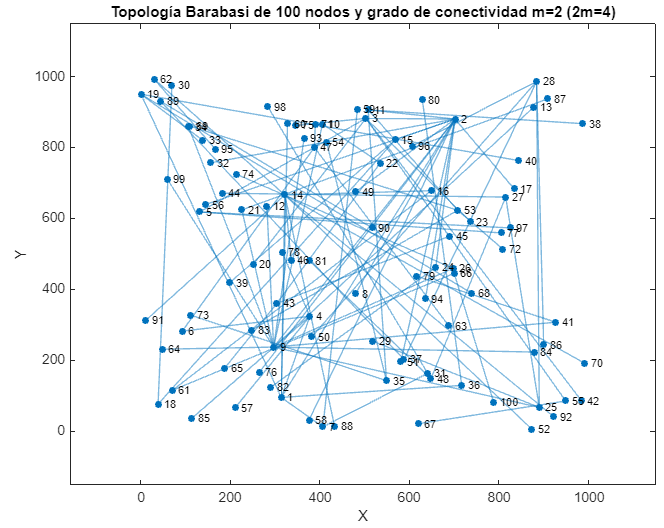
\includegraphics[width=\linewidth]{img/diseno/britebarabasi2.png}
      \label{fig:grafbrite1}
    \end{minipage}\hfill
    \begin{minipage}{0.5\textwidth}
      \centering
      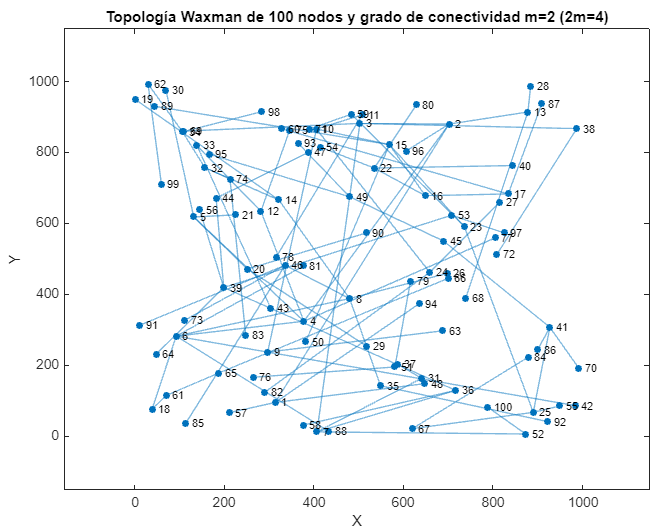
\includegraphics[width=\linewidth]{img/diseno/britewaxman2.png}
      \label{fig:grafbrite2}
    \end{minipage}\hfill
    \caption{Representación de diferencias de los modelos Router Barabasi-Albert y Waxman a partir de los mismos parámetros de entrada}
    \label{fig:grafbrite}
\end{figure}